\begin{enumerate}[label=\thesubsection.\arabic*.,ref=\thesubsection.\theenumi]
\numberwithin{equation}{enumi}

\item Sketch the Nyquist plot for a closed loop system having open-loop transfer function 
\begin{align}
\label{eq:ee18btech11035_GH}
    G\brak{s}H\brak{s}=\frac{2e^{-s\tau}}{s\brak{1+s}\brak{1+0.5s}}
\end{align}
Determine the maximum value of $\tau$ for the system to be stable.

\item Find $\text{Re} \cbrak{G(\j\omega)H(\j\omega)}$ and $\text{Im} \cbrak{G(\j\omega)H(\j\omega)}$.\\
\solution From \eqref{eq:ee18btech11035_GH},

\begin{multline}
\label{eq:ee18btech11035_Re}
\implies  \text{Re} \cbrak{G(\j\omega)H(\j\omega)} =
\\
-4\sbrak{\frac{3\omega^2\cos\brak{\omega\tau}-\brak{\omega^3-2\omega}\sin\brak{\omega\tau}}{  \brak{3\omega^2}^2+ \brak{\omega^3-2\omega}^2  }}
\end{multline}

\begin{multline}
\label{eq:ee18btech11035_Im}
\implies  \text{Im} \cbrak{G(\j\omega)H(\j\omega)} =
\\
4\sbrak{\frac{\brak{\omega^3-2\omega}\cos\brak{\omega\tau}+3\omega^2\sin\brak{\omega\tau}}{  \brak{3\omega^2}^2+ \brak{\omega^3-2\omega}^2  }}
\end{multline}

\item Determine the maximum value of $\tau$ for the system to be stable.\\
\solution Determining the stability of closed loop transfer function using Nyquist stability Criterion.\\
\begin{align}
    Z=P+N
\end{align}
Poles of open loop transfer function are on left half of s-plane.Therefore,$P=0$\\
To ensure that the system is stable $N$ should be 0\\
For maximum value of $\tau$ for stability ,the nyquist plot cuts the real axis at -1+j0.\\
\begin{align}
    G\brak{s}H\brak{s} &= -1+j0\\
    \label{eq:ee18btech11035_im0}
    \text{Im} \cbrak{G(\j\omega)H(\j\omega)} &= 0\\
    \label{eq:ee18btech11035_Re0}
    \text{Re} \cbrak{G(\j\omega)H(\j\omega)} &= -1
\end{align}

From \eqref{eq:ee18btech11035_Im} and \eqref{eq:ee18btech11035_im0}
\begin{align}
    \label{eq:ee18btech11035_tan}
    \implies \tan\brak{\omega\tau}&=\frac{-\brak{\omega^3-2\omega}}{3\omega^2}
\end{align}

From \eqref{eq:ee18btech11035_Re} and \eqref{eq:ee18btech11035_Re0} and substituting \tan\brak{\omega\tau}&=\frac{-\brak{\omega^3-2\omega}}{3\omega^2}


\begin{align}
    \label{eq:ee18btech11035_omega}
    \implies  \omega^6+5\omega^4+4\omega^2-16=0
\end{align}

Solving \eqref{eq:ee18btech11035_omega} graphically.\\

\begin{figure}[!h]
  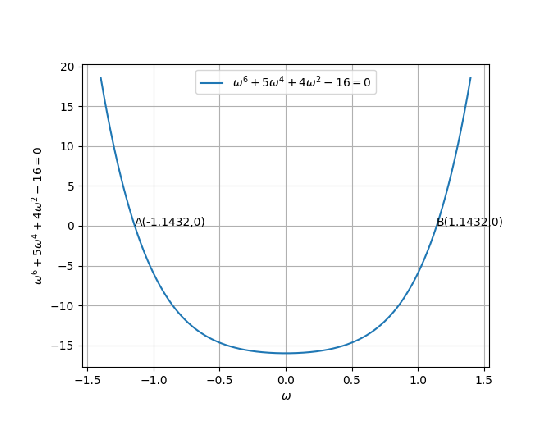
\includegraphics[width=\columnwidth]{./figs/ee18btech11035_1.eps}
  \caption{}
  \label{fig:ee18btech11035_1}
\end{figure}
Pyhton code for the above plot is
\begin{lstlisting}
codes/ee18btech11035_1.py
\end{lstlisting}

$\omega$ = 1.1432,-1.1432 \brak{As,\omega\text{ is positive}}\\
Therefore,$\omega$ = 1.1432\\

Substituting $\omega$ in \eqref{eq:ee18btech11035_tan}\\
\begin{align}
    \tan\brak{1.1432\tau}&=0.2021\\
    \tau&=0.1744
\end{align}

\item Sketch the Nyquist plot.
\\
\solution The following python code generates the Nyquist plot.
\begin{lstlisting}
codes/ee18btech11035_2.py
\end{lstlisting}

\begin{figure}[!h]
  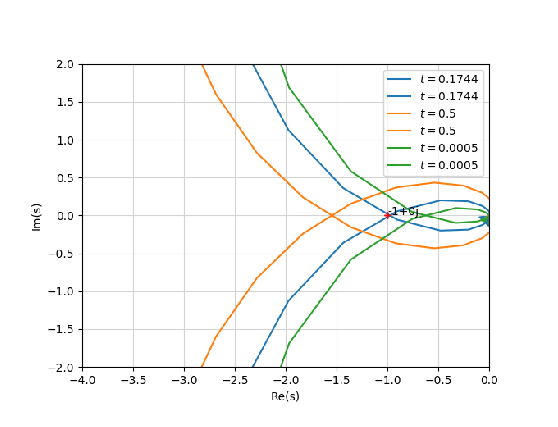
\includegraphics[width=\columnwidth]{./figs/ee18btech11035_2.eps}
  \caption{Nyquist plot for variable $\tau$}
  \label{fig:ee18btech11035_2}
\end{figure}

From the above figure \eqref{fig:ee18btech11035_2} $\tau \le 0.1744$ for a stable system.

\item Stability Criterion as varying $\tau$ 
\\
\solution 
\begin{table}[!ht]
\centering
\input{./tables/table.tex}
\caption{}
\label{table:ee18btech11035_table}
\end{table}

Therefore,$\tau_{max} = 0.1744 $\\.
\end{enumerate}
